\chapter[Results][Results]{Results}
\label{chap:results}

\begin{quote}
  Results of the $\Htautau$ analysis are described. This is described in additional detail in the recent ATLAS $\Htautau$ publication~\cite{HIGG-2013-32}. The description of the fit procedure draws heavily from the recent ATLAS $\HWW$ publication~\cite{HIGG-2013-13}.
\end{quote}

The yields of signal and background processes are extracted from a statistical analysis of the data and the predictions described in \cref{chap:strategy,chap:backgrounds}. A likelihood function is maximized which provides the ``best fit'' of the prediction to the data in each bin of the BDT discriminators within their prescribed uncertainties.

The likelihood contains the data and prediction from six signal regions: three final states and two categories. Control regions are also used to constrain some background uncertainties. For example, a region of data rich in top events is used in the $\tautaulh$ analysis to constrain the normalization on the portion of the top background predicted with simulation.

\section{Fit procedure}
\label{sec:results-fit-procedure}

The statistical analysis maximizes a likelihood function $\Lang$ which depends on the signal strength $\upmu$, the set of uncertainties (or nuisance parameters) $\theta_i$, and the observed number of data events $N$. The signal strength is defined as the measured $\Htautau$ cross-section divided by the predicted $\Htautau$ cross-section. A measured $\upmu=1$ would imply exactly the same number of $\Htautau$ events are observed as expected.

\subsection{Likelihood function}

The likelihood function is shown in \cref{fig:results-likelihood-eqn}. It is the product of four terms.
%
%% \begin{description}
%%     \item[Observed data in the signal region bins:] \hfill \\
%%       Poisson function $f\left(N \ | \ \sig + \bkg\right)$ for the probability of observing $N$ events given a prediction $\sig + \bkg$ in each BDT bin

%%     \item[Observed data in the control regions:] \hfill \\
%%       Poisson function $f\left(N \ | \ \bkg\right)$ for the probability of observing $N$ events given a prediction $\bkg$ in each control region

%%     \item[Gaussian uncertainties:] \hfill \\
%%       Unit Gaussian function $g$ representing the systematic uncertainties. The mean and standard deviation are defined to be 0 and 1, respectively.

%%     \item[Prediction sample statistics:] \hfill \\
%%       Poisson function $f$ representing the statistical uncertainties given the finite sample size of the predictions

%% \end{description}
%

\begin{figure}[tp]
  \centering
  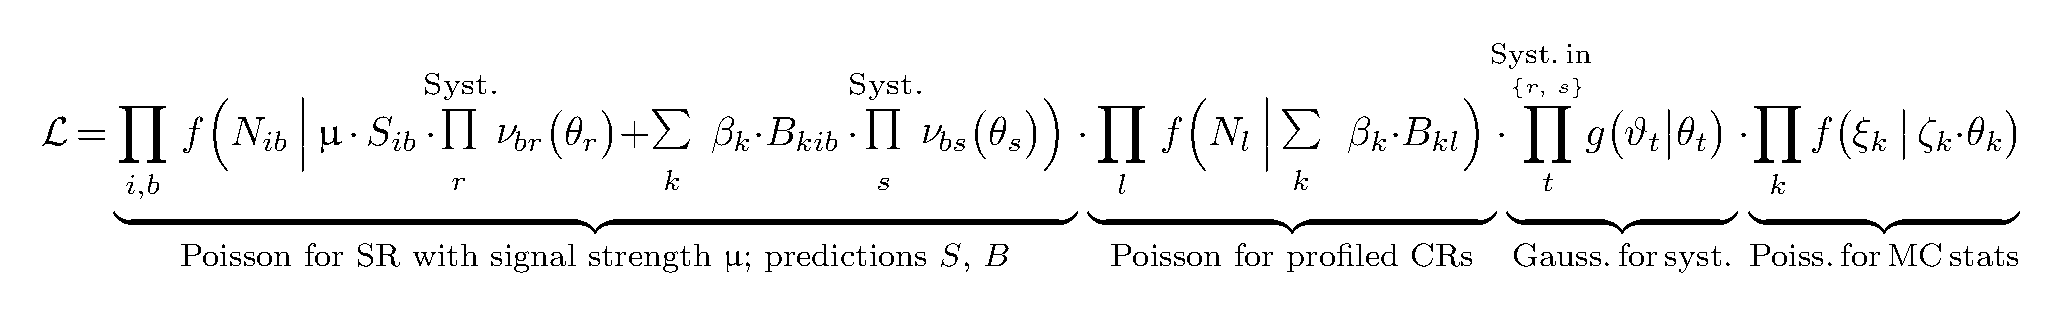
\includegraphics[width=0.99\textwidth]{figures/likelihood/equation}
  \caption{The likelihood equation considered for maximization~\cite{HIGG-2013-13}.}
  \label{fig:results-likelihood-eqn}
\end{figure}

The first term of the likelihood is a Poisson function, in each bin \textit{b} of each category \textit{i}, describing the probability of observing $N$ events given the predicted number of signal events $S$ and background events $B$. The number of signal events is scaled by the signal strength $\upmu$ which is shared among bins and categories. The number of background events is scaled by a parameter $\beta_k$ which can be category-dependent. The signal and background predictions are modified by response functions $\nu(\theta)$ for each nuisance parameter $\theta$. 

The response function for bin-wise systematic uncertainties is given by $\nu(\theta) = 1 + \theta\cdot\frac{\Delta_\theta}{N}$, where $\Delta_\theta$ is the given uncertainty on $\theta$ in units of $N$, i.e., $N\cdot\nu(\theta = \pm 1) = N \pm \Delta_\theta$ for $N=S,B$. The response function for statistical uncertainties on the predictions is $\nu(\theta) = \theta$.

The second term is a Poisson function, in each control region \textit{l}, describing the probability of observing $N$ events given the predicted number of background events $B$. The number of background events is scaled by a parameter $\beta_k$ which is shared with the first term. The statistical power of the control region data is then used to constrain the background normalization in the signal region.

The third term is a Gaussian function, for each systematic uncertainty, describing the probability of a given nuisance parameter being pulled away from its nominal value. This is a penalty term for choosing a less likely value of the nuisance parameter than the nominal value. The choice of Gaussian function to describe the uncertainty is convention.

The fourth term is a Poisson function, in each bin of each category, describing the uncertainty due to finite sample size of the signal and background predictions. This is especially relevant for predictions which have natural statistical limitations, e.g., predicting the $\Ztautau$ background with $\Zmumu$ events from data.

To extract the observed $\upmu$ and other quantities, the likelihood is maximized with respect to $\upmu$ and the associated nuisance parameters $\theta$. This maximization yields the most probable $\upmu$. The likelihood is evaluated at $\vartheta = 0$ and $\xi = \zeta$ which imposes that the most probable value of each systematic nuisance parameter is zero and statistical nuisance parameter is one.

\subsection{Features}

The first term of the likelihood is maximized when the prediction exactly matches the observed data events in a given bin. The prediction is allowed to change within the maximization as the nuisance parameters are pulled. This allowed change is restricted by the Gaussian constraints imposed on these uncertainties, which are maximized when the nuisance parameters are unchanged from their pre-fit prediction. For example, the jet energy scale is allowed to be moved by $+1\sigma$, but this incurs a penalty in the likelihood of $\frac{g(1|0,1)}{g(0|0,1)}\approx 0.6$. 

The normalization of the embedded $\Ztautau$ is allowed to float freely within each final state, i.e., there is no constraint beyond the signal region statistics. In the $\tautaulh$ channel, a single normalization nuisance parameter is used for $\Ztautau$ which is shared in each BDT bin of each category. This is sensible because the defining features of the categories -- dijet kinematics and $\pt^Z$ -- are expected to be well predicted by the embedding method.

The likelihood maximization extracts many fitted parameters, including the signal strength $\upmu$, the pulls of the nuisance parameters $\theta_i$, and the uncertainties on the nuisance parameters in units of the pre-fit uncertainties (i.e., $\Delta_{\theta,\text{pre-fit}} = 1$).

\subsection{Test statistic}

The test statistic is defined as:
%
\begin{equation}
  \begin{split}
    q(\upmu) &= -2\ \text{ln} \left(\frac{\Lang(\upmu, \theta_i)}{\Lang_\text{max.}}\right) \Bigg\rvert_{\theta_i = \hat{\theta}_{i,\upmu}} \\
  \end{split}
  \label{eqn:test-statistic}
\end{equation}
%
and is evaluated as a function of $\upmu$. The denominator $\Lang_\text{max.}$ is the unconditional maximum of the likelihood as a function of $\upmu$ and the nuisance parameters $\theta_i$ and is therefore just a number. The numerator $\Lang(\upmu, \theta_i)$ is the conditional maximum for a given $\upmu$ as a function of the nuisance parameters, thereby asking which signal strength is most likely.

The fitted uncertainty on a nuisance parameter is defined as the distance $\theta_\text{right} - \theta_\text{left}$ such that $q(\upmu) = 1$ when scanning a given nuisance parameter to the right and left of the fitted $\theta$. If $\Lang$ follows a Gaussian distribution, the integral from $\theta_\text{left}$ to $\theta_\text{right}$ corresponds to 68\% ($1\sigma$) of the distribution.

\subsection{Impact of uncertainties on $\upmu$}

The post-fit \textit{impact} of a given nuisance parameter on the signal strength is defined as:
%
\begin{equation}
  \begin{split}
    \Delta_{\hat{\upmu}, i} &= \hat{\upmu}\left(\hat{\theta}_i \pm \Delta_{\hat{\theta}_i}\right) - \hat{\upmu} \\
  \end{split}
  \label{eqn:impact}
\end{equation}
%
where hats indicate post-fit values. $\hat{\upmu}\left(\hat{\theta}_i \pm \Delta_{\hat{\theta}_i}\right)$ indicates the fitted $\upmu$ of the full fit but with $\theta_i$ fixed to its post-fit value $\hat{\theta}$ varied by the post-fit uncertainty $\pm\Delta_{\hat{\theta}, i}$, where all other nuisance parameters are floating. If the fitted $\upmu$ is robust against changes to a nuisance parameter, its impact will be small.

\section{Fit results}
\label{sec:results-fit-results}

The data and fitted signal and background predictions are shown in \cref{fig:results-bdts}. The majority of bins in the BDTs are dominated by background, and good modeling is observed. In the signal-like regime of BDT output near 1, the predicted contribution from $\Htautau$ signal is visible in the VBF category of each final state, and the signal hypothesis is favored over the background-only hypothesis.

The yields in the VBF $\Htautaulh$ category and in the most signal-like regime are shown in \cref{tab:results-yields} after the global fit. In the highest BDT bin, the signal hypothesis is favored over the background-only hypothesis.

\begin{table}[bp] 
  \centering
  \renewcommand{\arraystretch}{1.4}
  \caption{Data and the predicted yields of signal and background in the VBF $\tautaulh$ category after the global fit.}
  \begin{tabular}{l|ccc}
  Process/Category  & \multicolumn{3}{c}{VBF $\tautaulh$} \\
  \hline
  BDT output bin    & All bins      & Second to last bin & Last bin    \\
  \hline
  $\fakes$          & $1680 \pm 50$ & $ 8.2 \pm 0.9$ & $5.2  \pm 0.7$  \\
  $\Ztautau$        & $ 877 \pm 29$ & $ 7.6 \pm 0.9$ & $4.2  \pm 0.7$  \\
  Top               & $  82 \pm 15$ & $ 0.3 \pm 0.4$ & $0.5  \pm 0.4$  \\
  $\Zll$ $(\lfake)$ & $  54 \pm 26$ & $ 1.0 \pm 0.7$ & $0.30 \pm 0.28$ \\
  Diboson           & $  63 \pm 11$ & $ 1.0 \pm 0.4$ & $0.48 \pm 0.20$ \\
  \hline
  ggF $\Htautau$    & $  16 \pm 6$  & $ 1.0 \pm 0.4$ & $1.2  \pm 0.6$  \\
  VBF $\Htautau$    & $  31 \pm 8$  & $ 4.5 \pm 1.1$ & $9.1  \pm 2.2$  \\
  $W\Htautau$       & $ < 1$        & $< 0.1$        & $< 0.1$         \\
  $Z\Htautau$       & $ < 1$        & $< 0.1$        & $< 0.1$         \\
  \hline
  Total background  & $2760 \pm 40$ & $18.1 \pm 2.3$ & $10.7 \pm 2.7$  \\
  Total signal      & $  48 \pm 12$ & $ 5.5 \pm 1.3$ & $10.3 \pm 2.5$  \\
  \hline
  Data              & 2830          & 22             & 21             \\
\end{tabular}


  \label{tab:results-yields}
\end{table}

At the value of the Higgs boson mass obtained from the combination of the ATLAS $\Hyy$ and $\HZZ$ measurements, the signal strength obtained is $1.4 \pm 0.3 \text{ (syst.)} \pm 0.3 \text{ (stat.)} \pm 0.1 \text{ (theo.)}$. The signal strength breakdown by category and channel is shown in \cref{fig:results-musummary}.

The probability $p_0$ of obtaining a result at least as signal-like as observed in the data if no signal were present is calculated using the test statistic $q(0)$. For $m_H = 125.36$ GeV, the observed $p_0$ is $2.7 \times 10^{-6}$, which corresponds to a deviation from the background-only hypothesis of 4.5$\sigma$.  This can be compared to an expected significance of 3.4$\sigma$.

To emphasize the most signal-like regime, two distributions are built from the six categories used in the global fit and shown in \cref{fig:results-money-plots}. First, the signal region bins of the BDT discriminator are re-ordered by $\log_{10}(S/B)$, where $S/B$ is the signal-to-background ratio calculated assuming $\upmu=1.4$ in each bin. The expected signal yield for both $\upmu=1$ and $\upmu=1.4$ is shown, as well as the fitted background yield for the background-only hypothesis. The signal hypothesis is clearly favored. Second, the $\mMMC$ distribution is shown summed across all categories and weighted event-by-event by $\ln(1+S/B)$, which enhances the events compatible with the signal hypothesis. The excess of events in this mass distribution is consistent with the expectation for a Standard Model Higgs boson with $m_H = 125$ GeV.

\clearpage
\begin{figure}[tp]
  \centering
  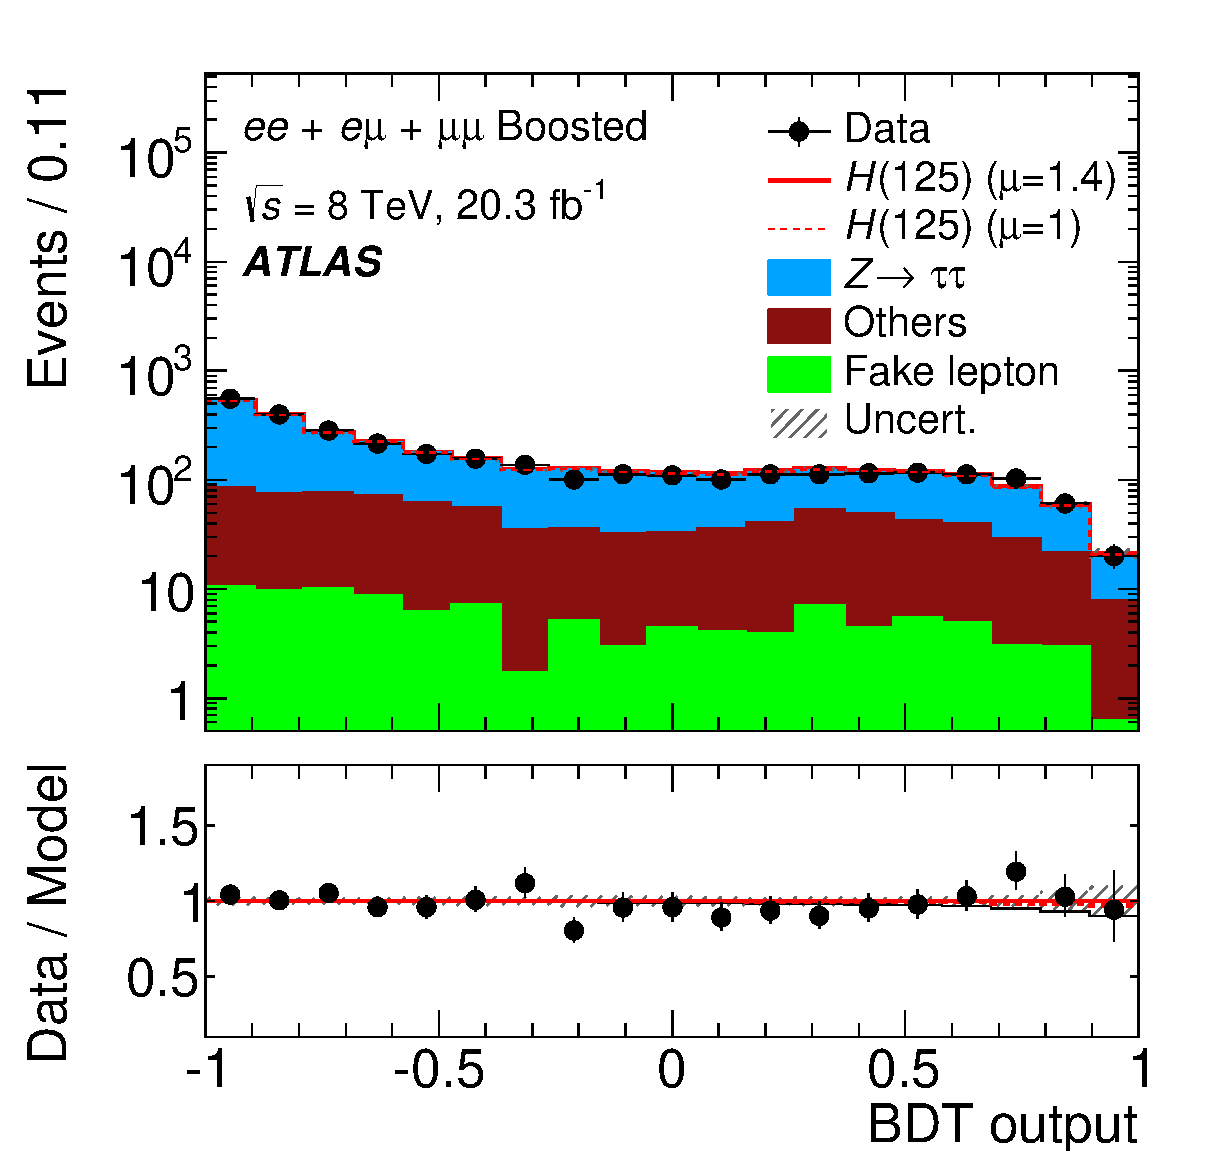
\includegraphics[width=0.45\textwidth]{figures/HIGG-2013-32/fig_08b}
  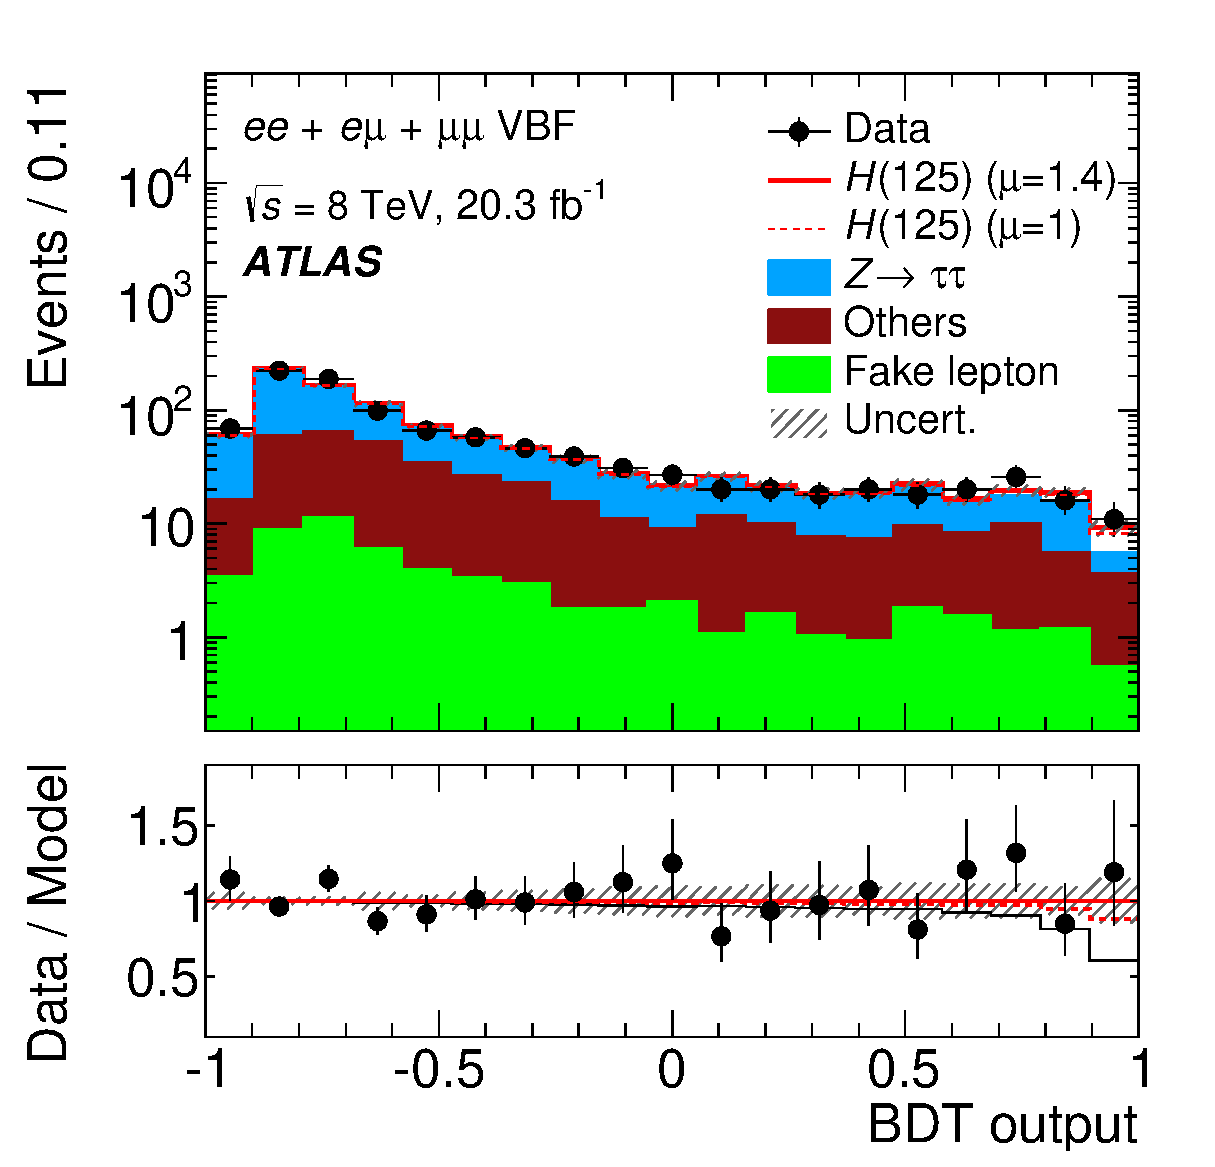
\includegraphics[width=0.45\textwidth]{figures/HIGG-2013-32/fig_08a}
  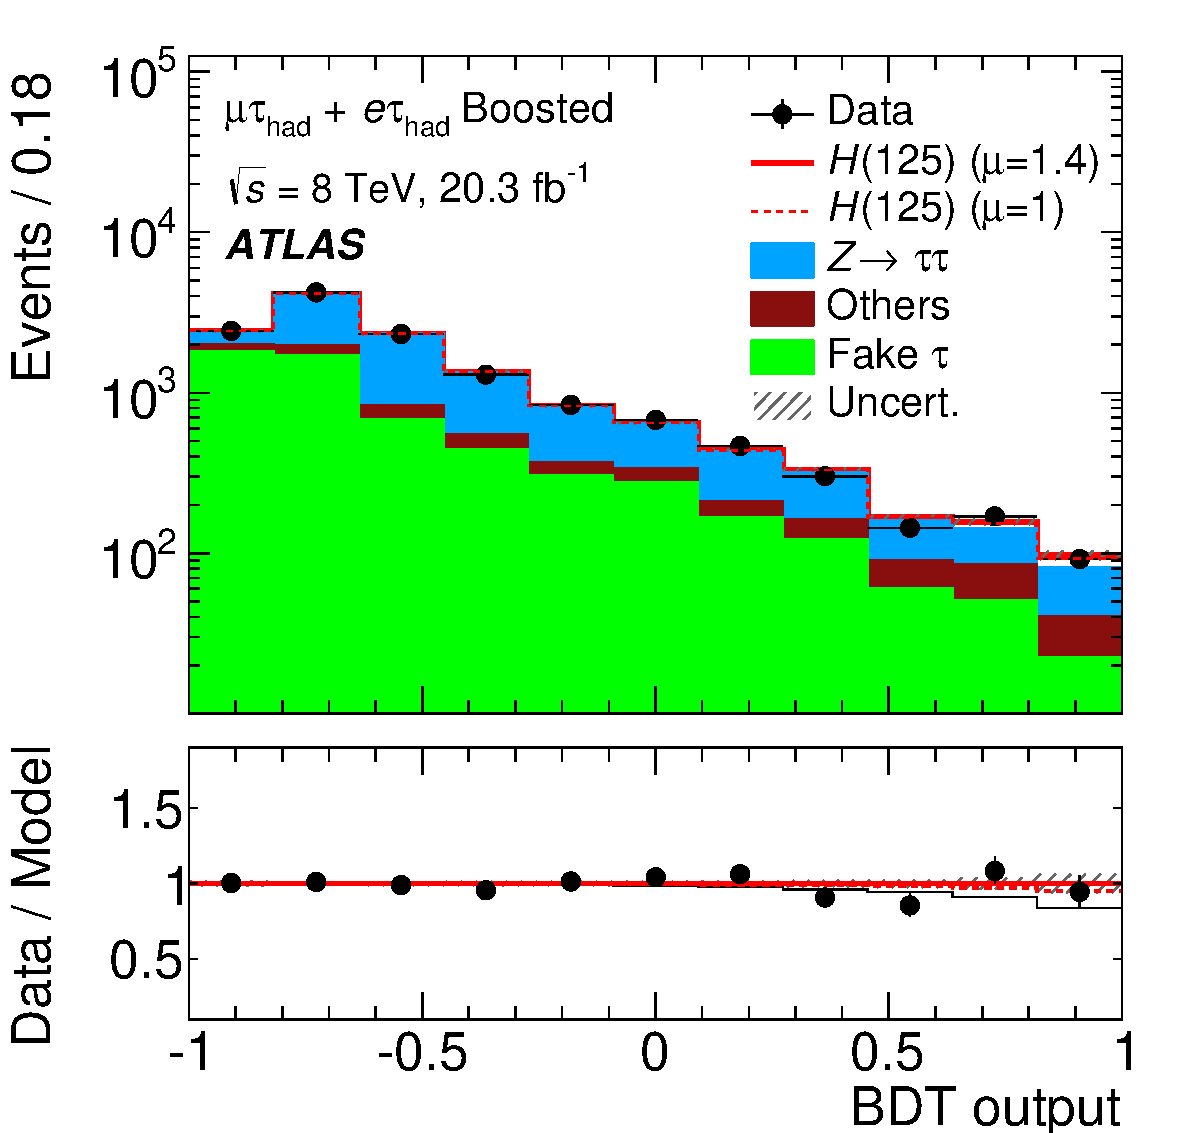
\includegraphics[width=0.45\textwidth]{figures/HIGG-2013-32/fig_08d}
  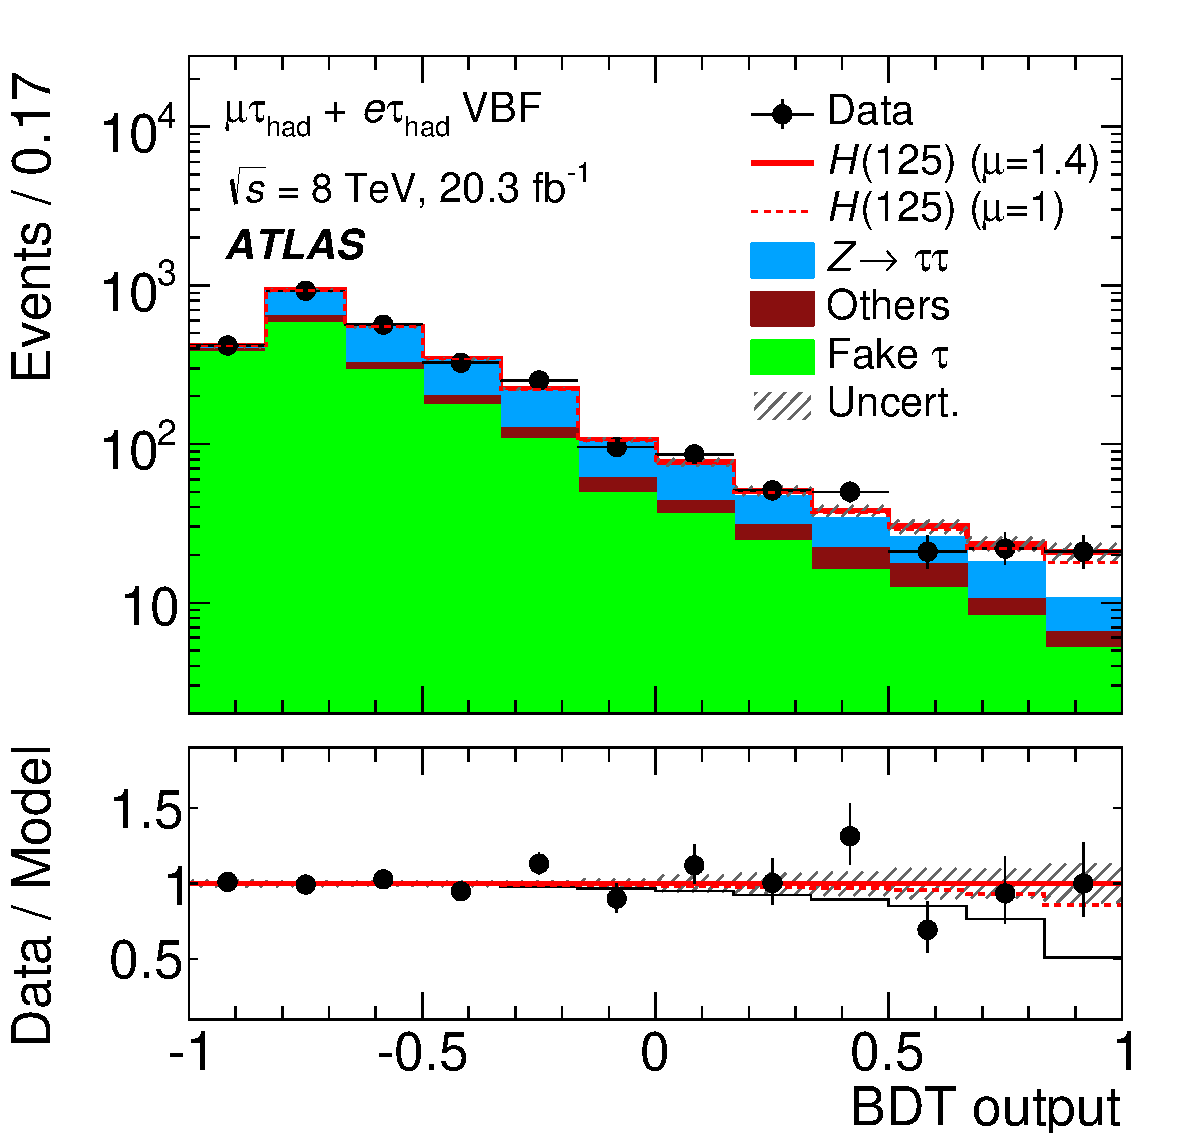
\includegraphics[width=0.45\textwidth]{figures/HIGG-2013-32/fig_08c}
  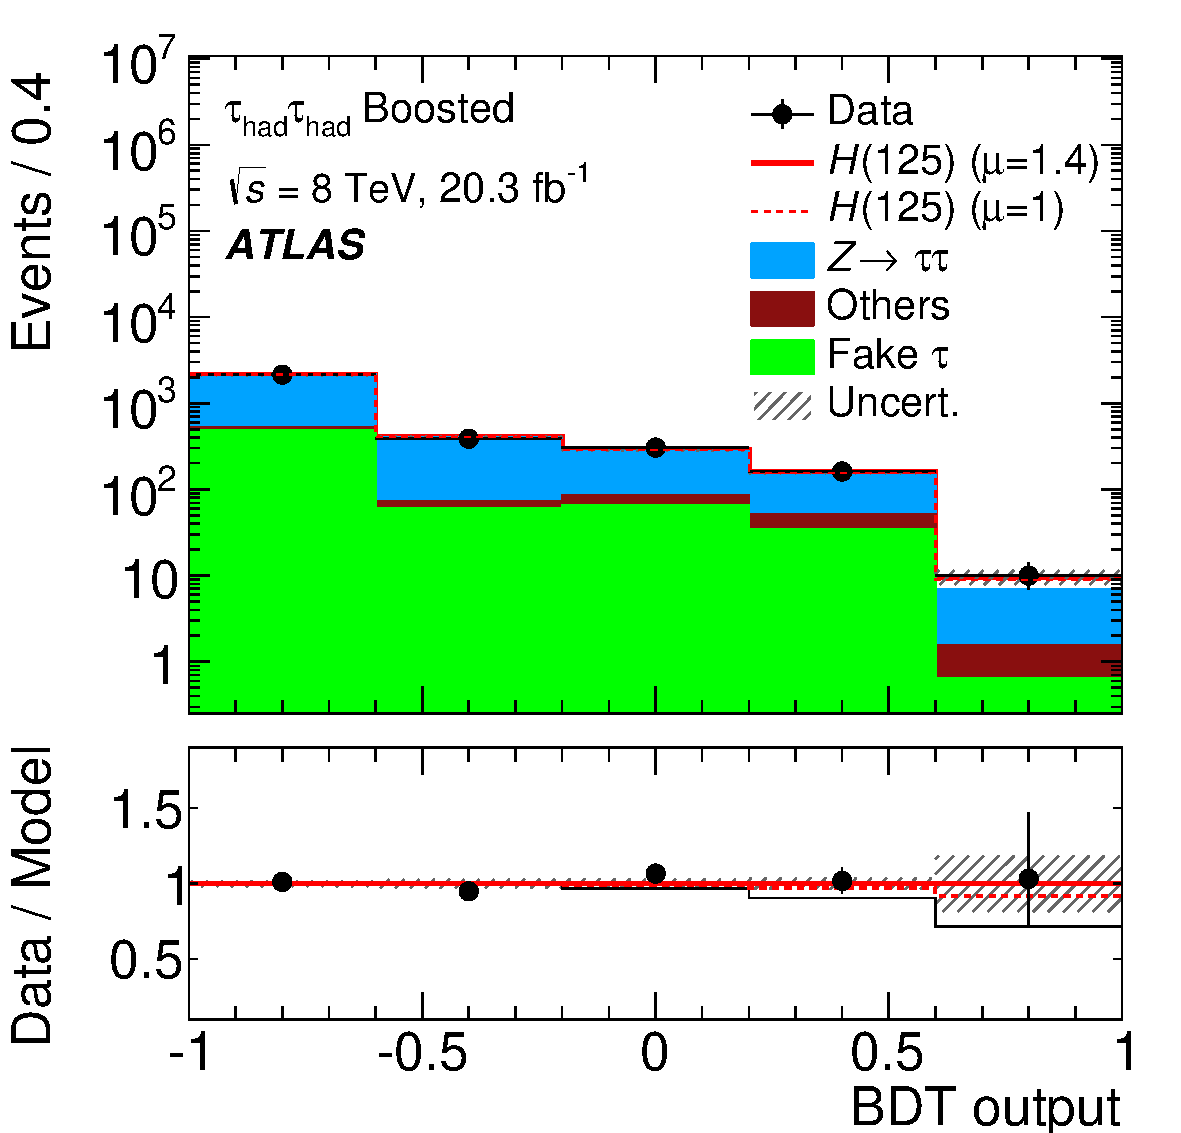
\includegraphics[width=0.45\textwidth]{figures/HIGG-2013-32/fig_08f}
  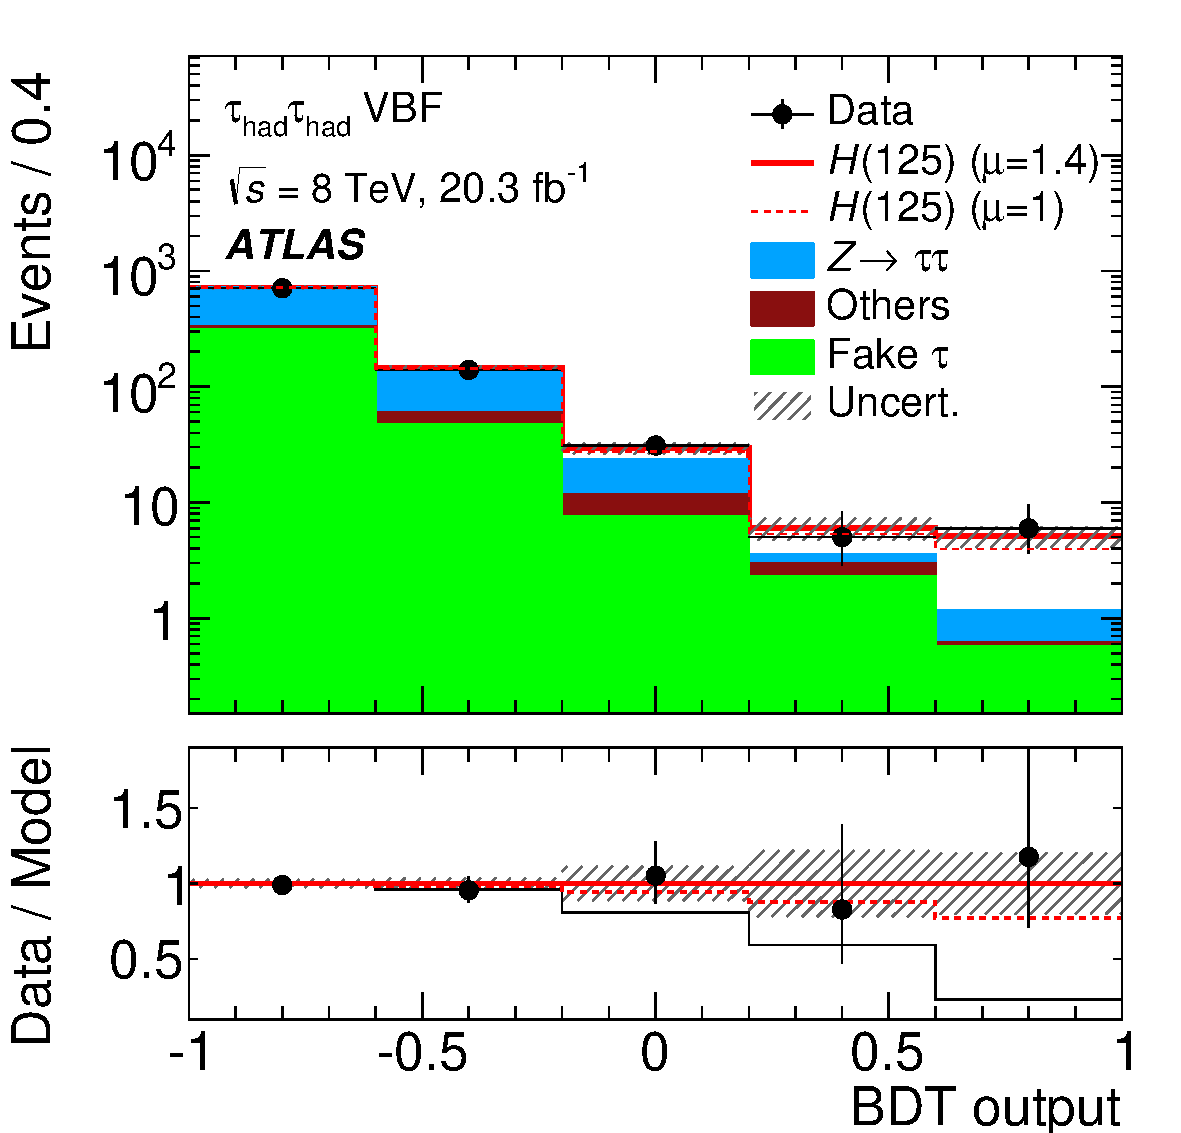
\includegraphics[width=0.45\textwidth]{figures/HIGG-2013-32/fig_08e}
  \caption{Distributions of the 8 TeV BDT discriminants in all six analysis categories after the global fit~\cite{HIGG-2013-32}.}
  \label{fig:results-bdts}
\end{figure}
\clearpage

\begin{figure}[tp]
  \centering
  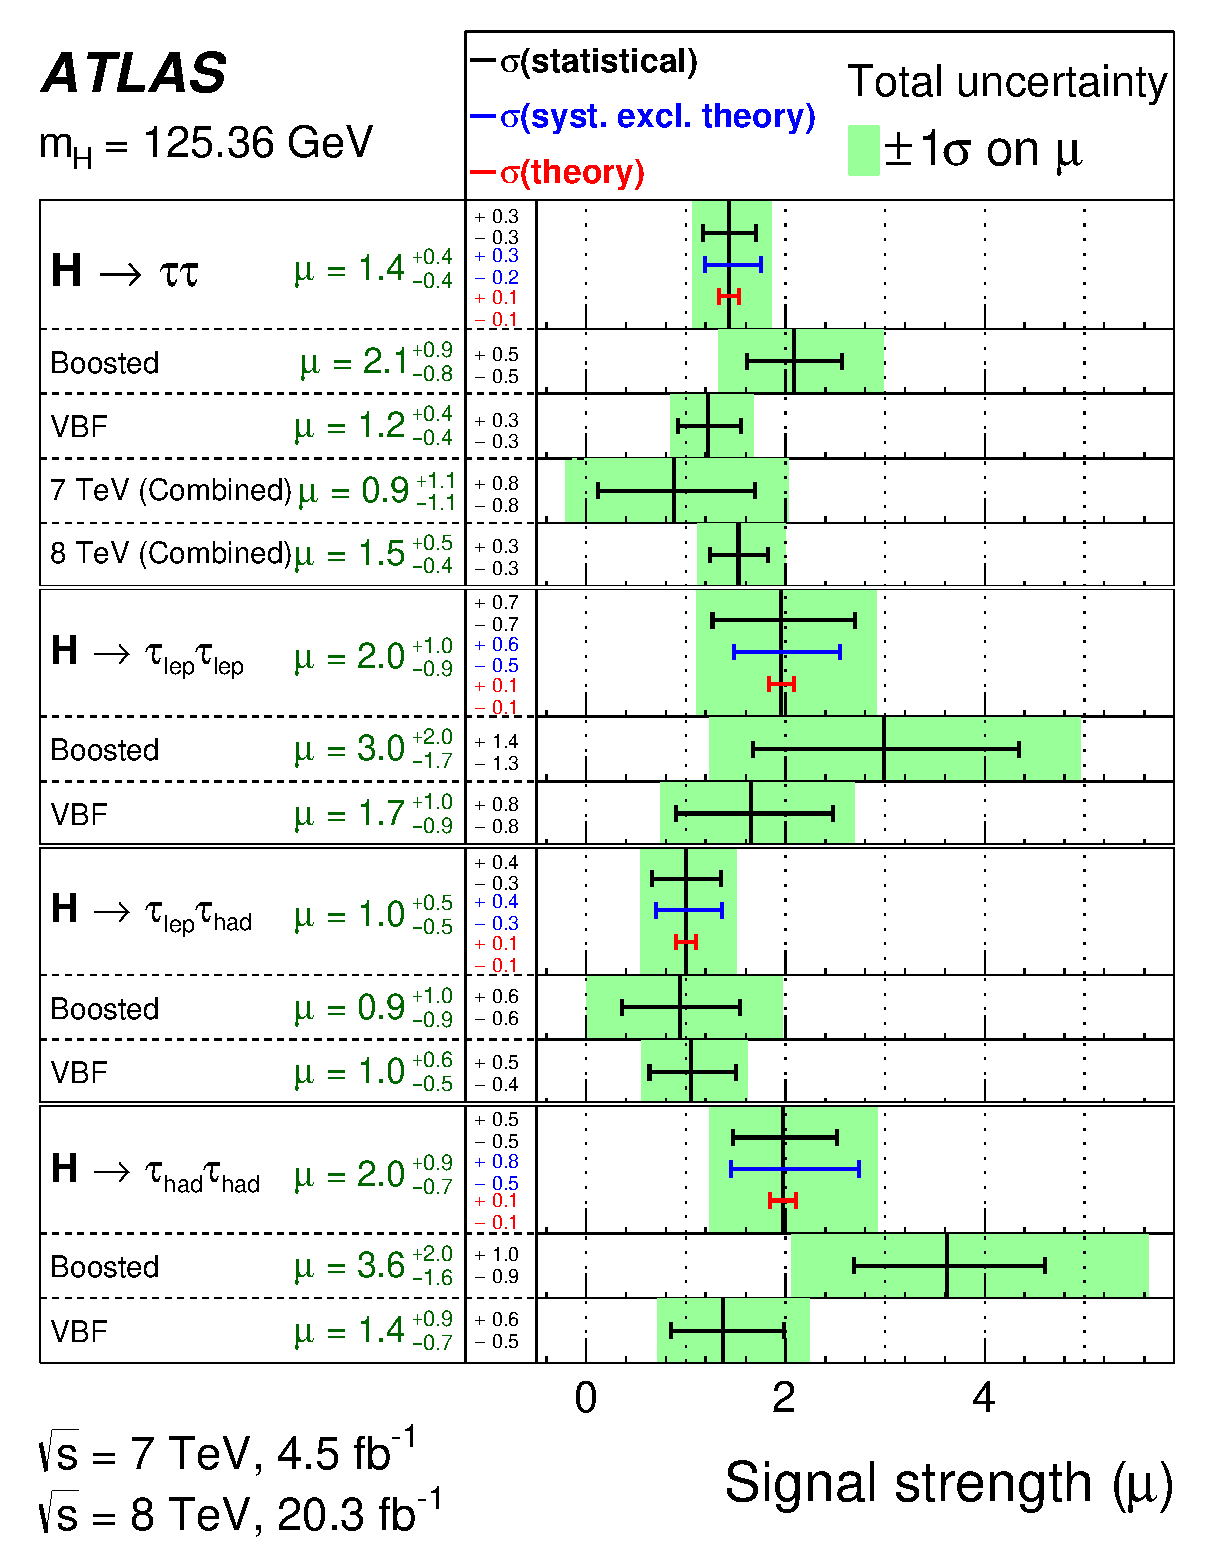
\includegraphics[width=0.90\textwidth]{figures/HIGG-2013-32/fig_09}
  \caption{The fitted signal strength $\upmu$ split by category, final state, and data-taking period~\cite{HIGG-2013-32}.}
  \label{fig:results-musummary}
\end{figure}

\begin{figure}[tp]
  \centering
  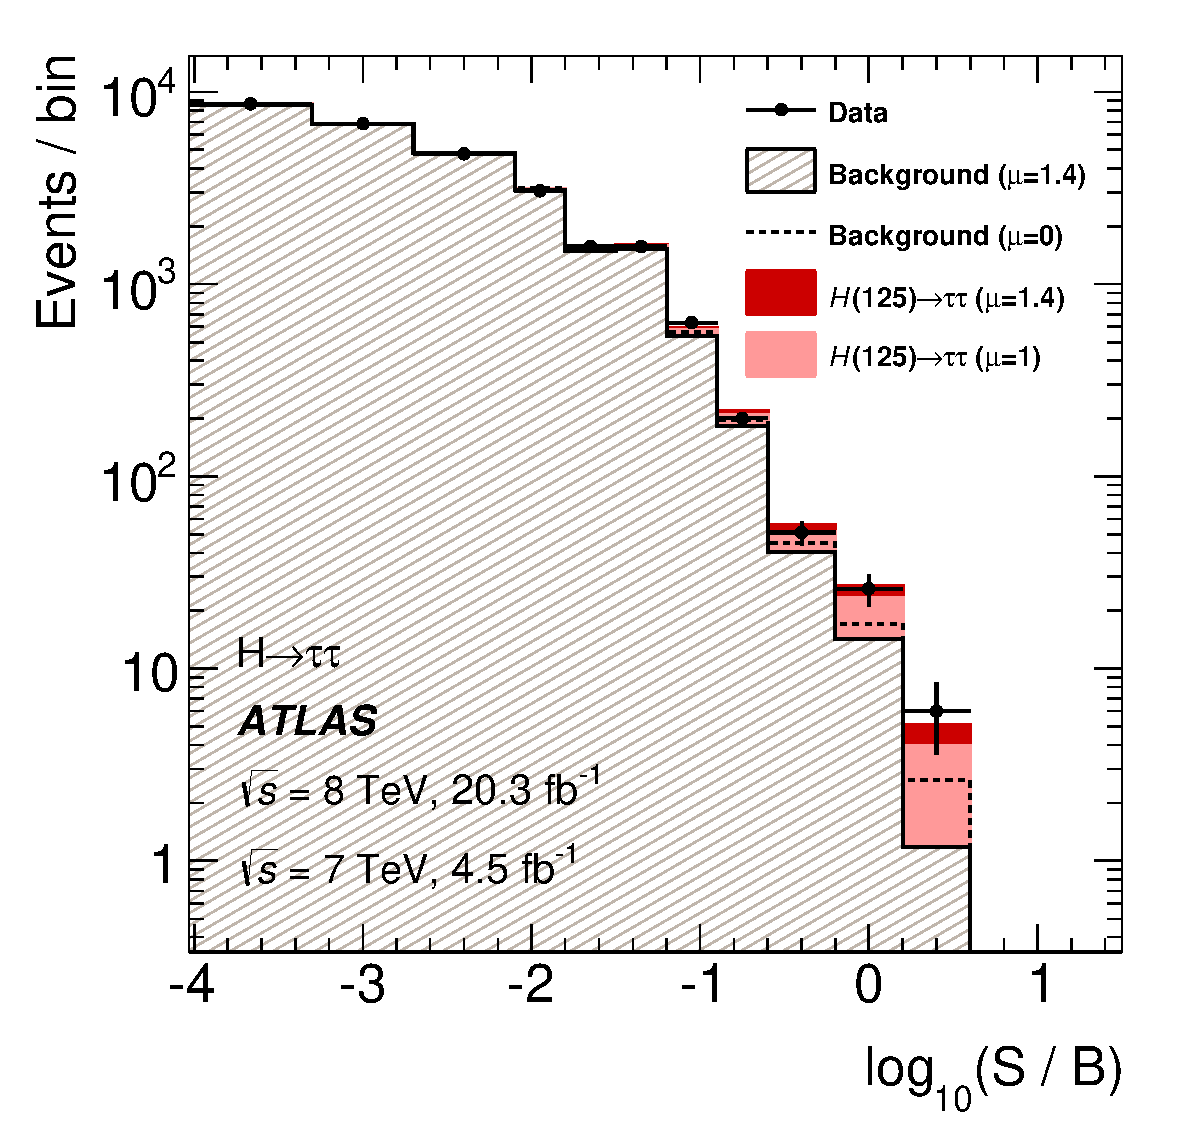
\includegraphics[width=0.45\textwidth]{figures/HIGG-2013-32/fig_10}
  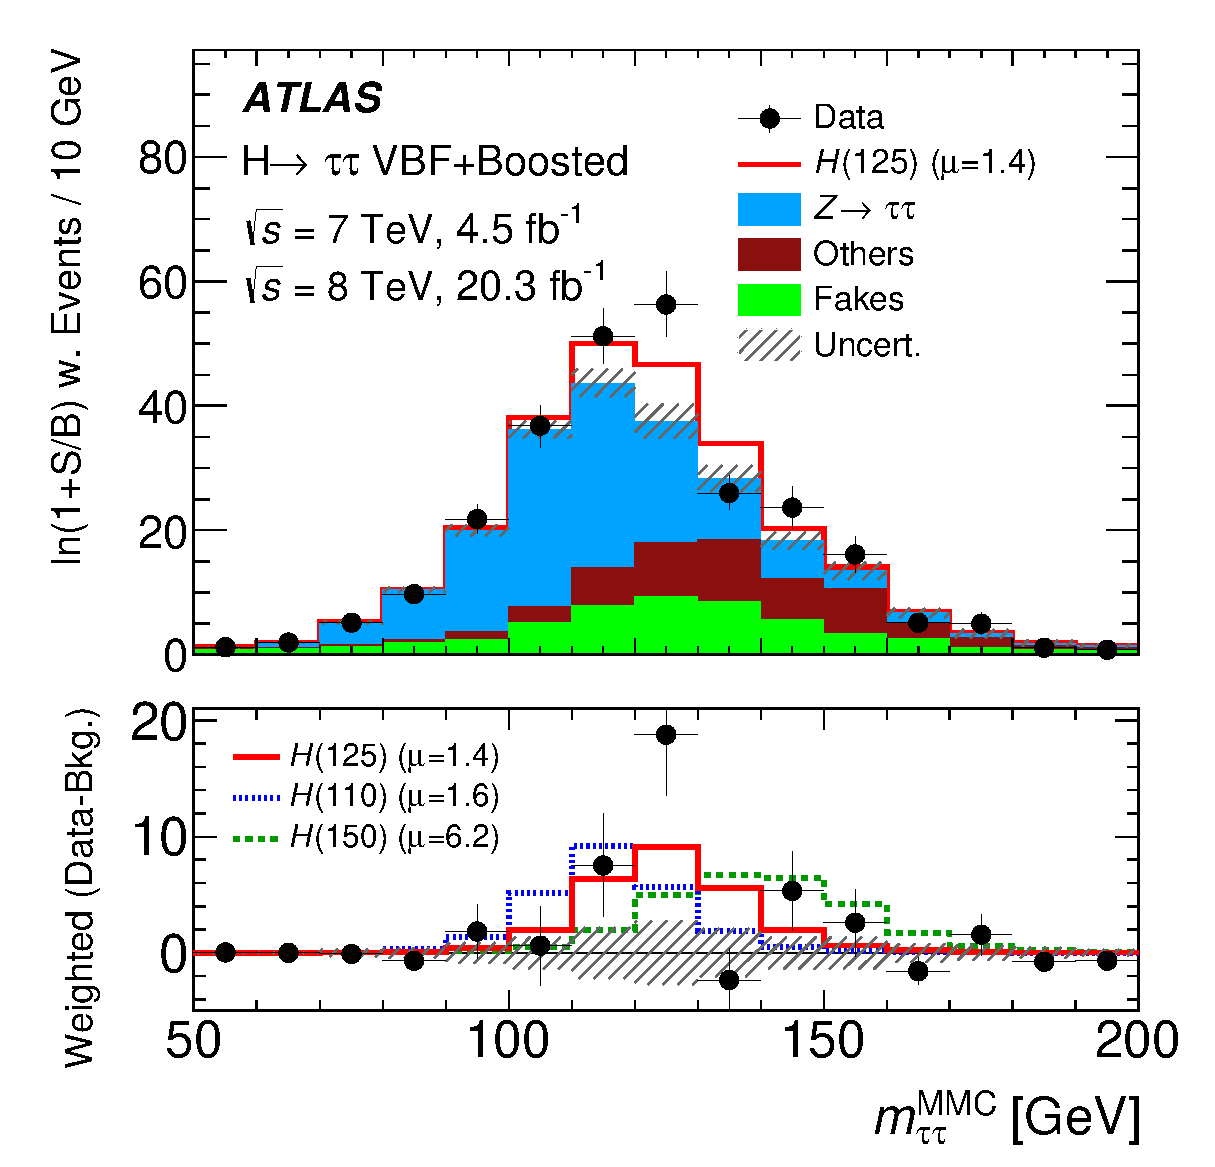
\includegraphics[width=0.45\textwidth]{figures/HIGG-2013-32/fig_11b}
  \caption{Plots of data and prediction which emphasize the most sensitive regions~\cite{HIGG-2013-32}. The individual BDT bins from all six categories are ordered by S/B and plotted on a shared axis (left) and entries in the $\mMMC$ distribution are weighted by $\text{log}(1+S/B)$ (right).}
  \label{fig:results-money-plots}
\end{figure}

The dominant uncertainties on the measurement of the signal strength parameters include statistical uncertainties on the data from the signal regions, uncertainties on the jet and tau energy scales, uncertainties on the normalization of the $\Ztautau$ and top backgrounds, and theoretical uncertainties. The contributions of each of these significant sources to the uncertainty of the measured signal strength are summarized in \cref{fig:results-uncertainties-1}.

\begin{figure}[tp]
  \centering
  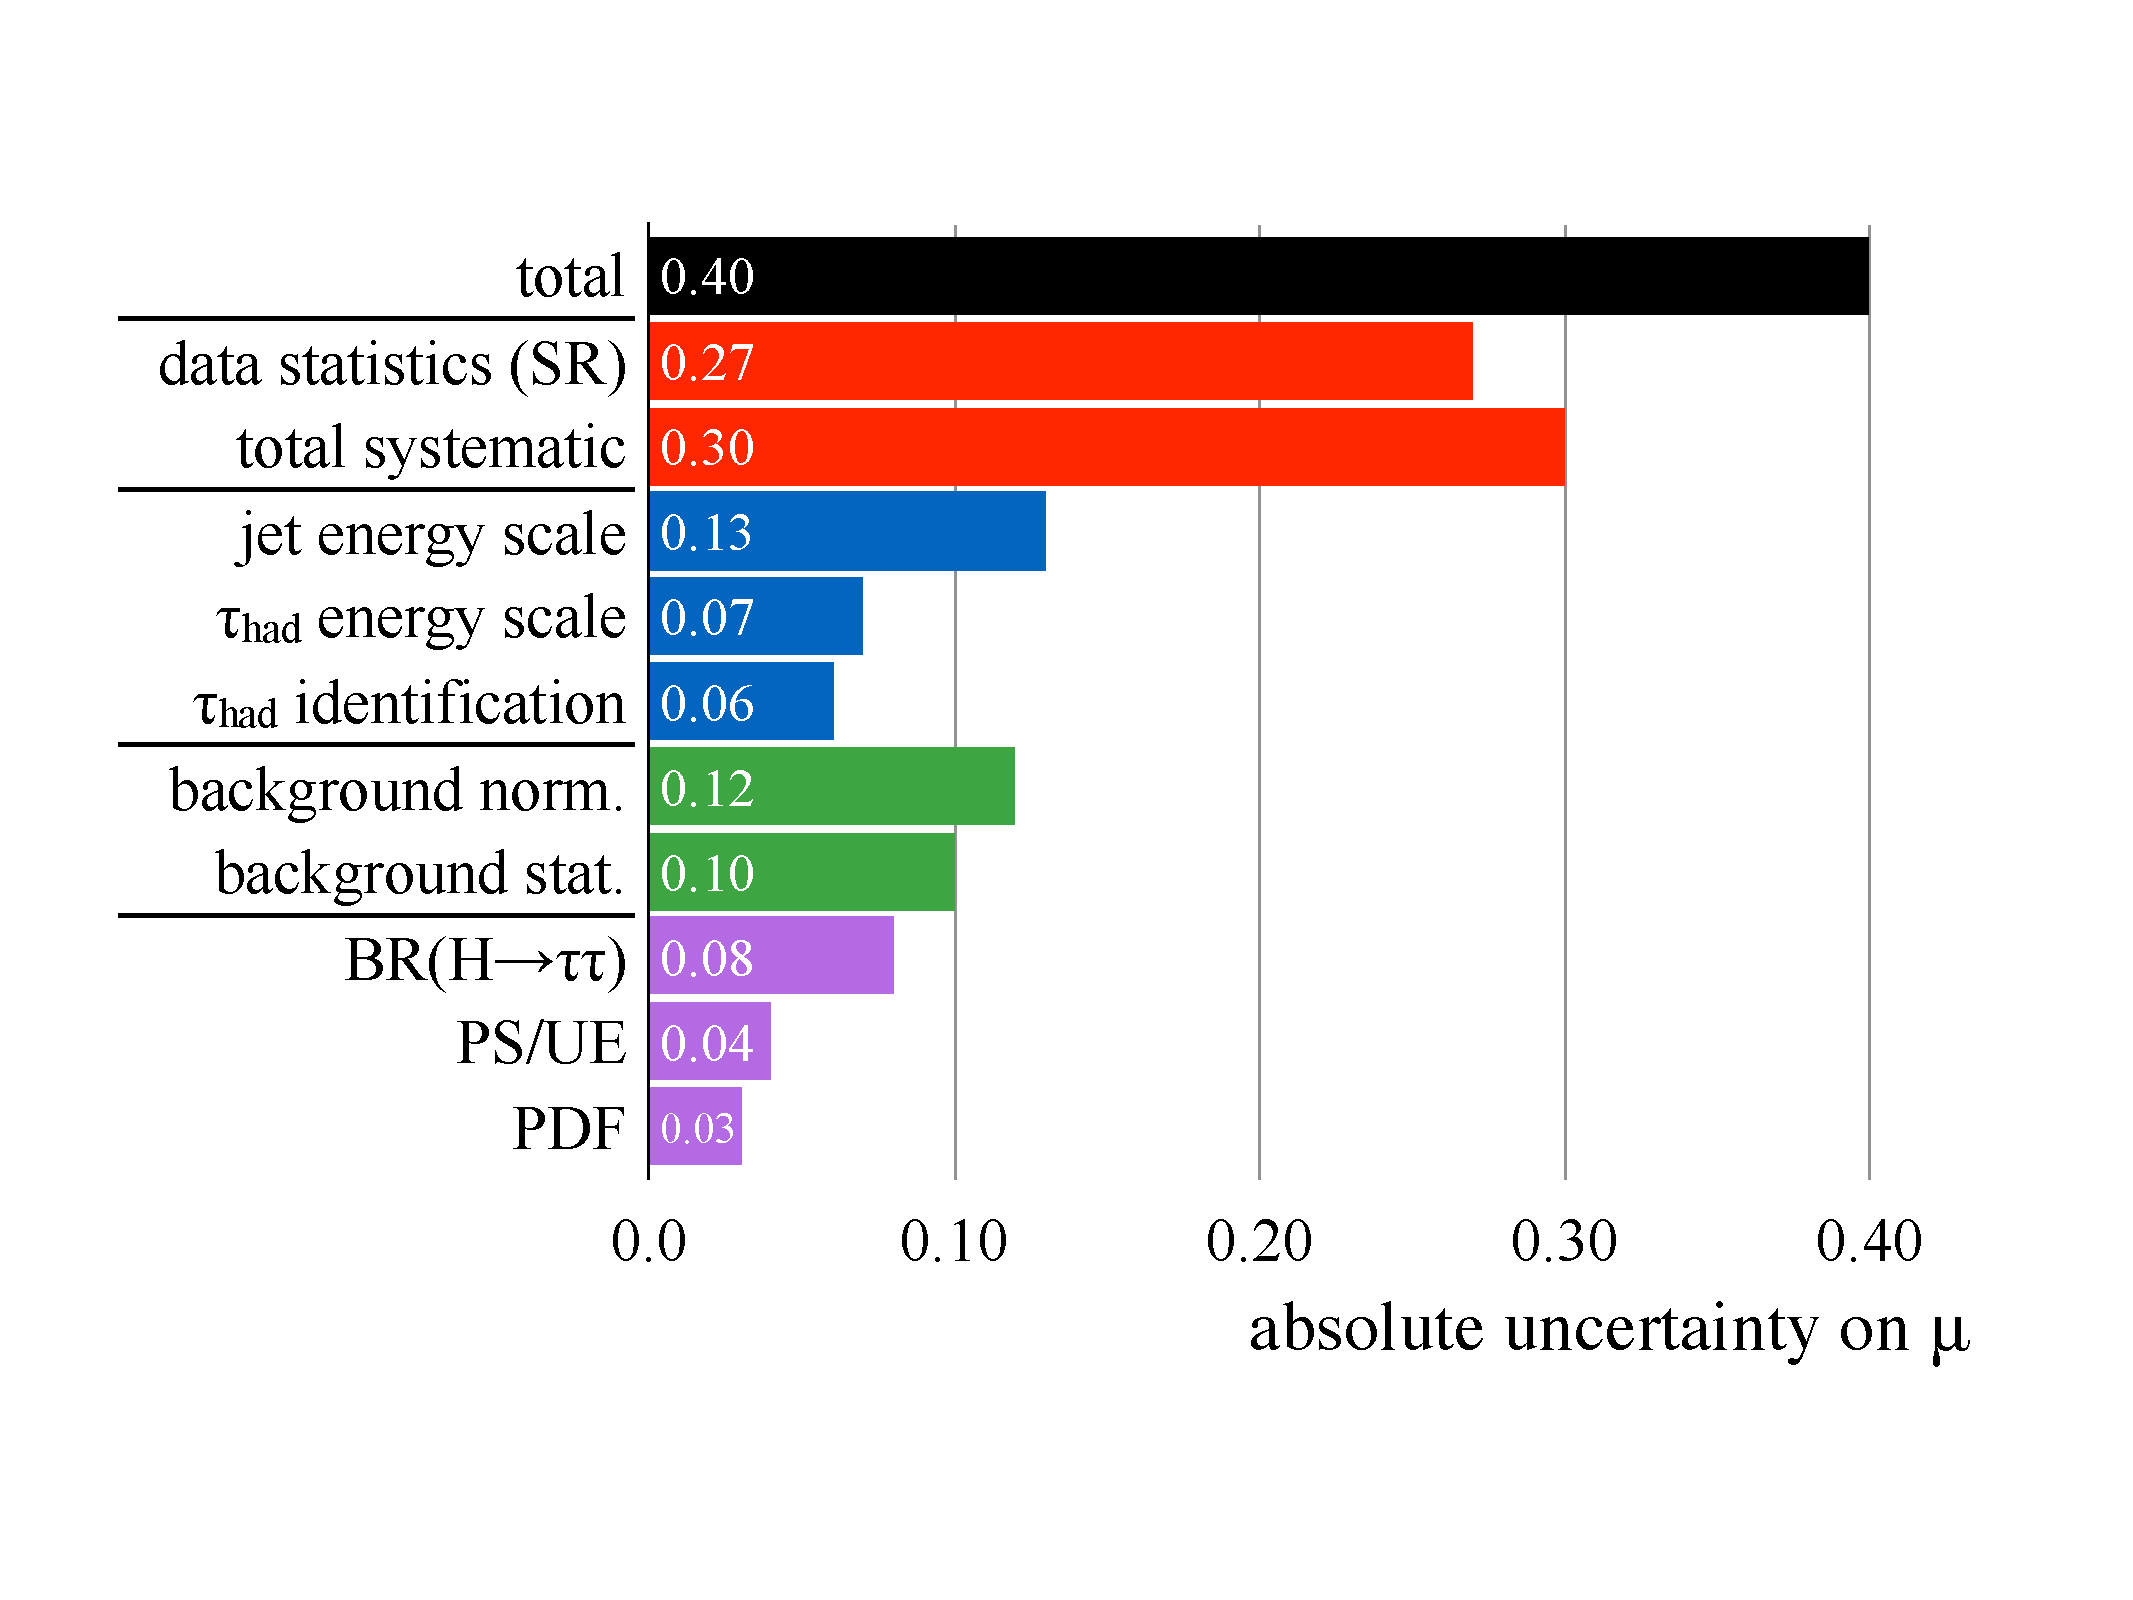
\includegraphics[width=0.90\textwidth]{figures/HIGG-2013-32/uncertainties}
  \caption{Comparison of the impact of the statistical and systematic uncertainties on the absolute uncertainty on $\upmu$~\cite{HIGG-2013-32}.}
  \label{fig:results-uncertainties-1}
\end{figure}

%% \begin{figure}[tp]
%%   \centering
%%   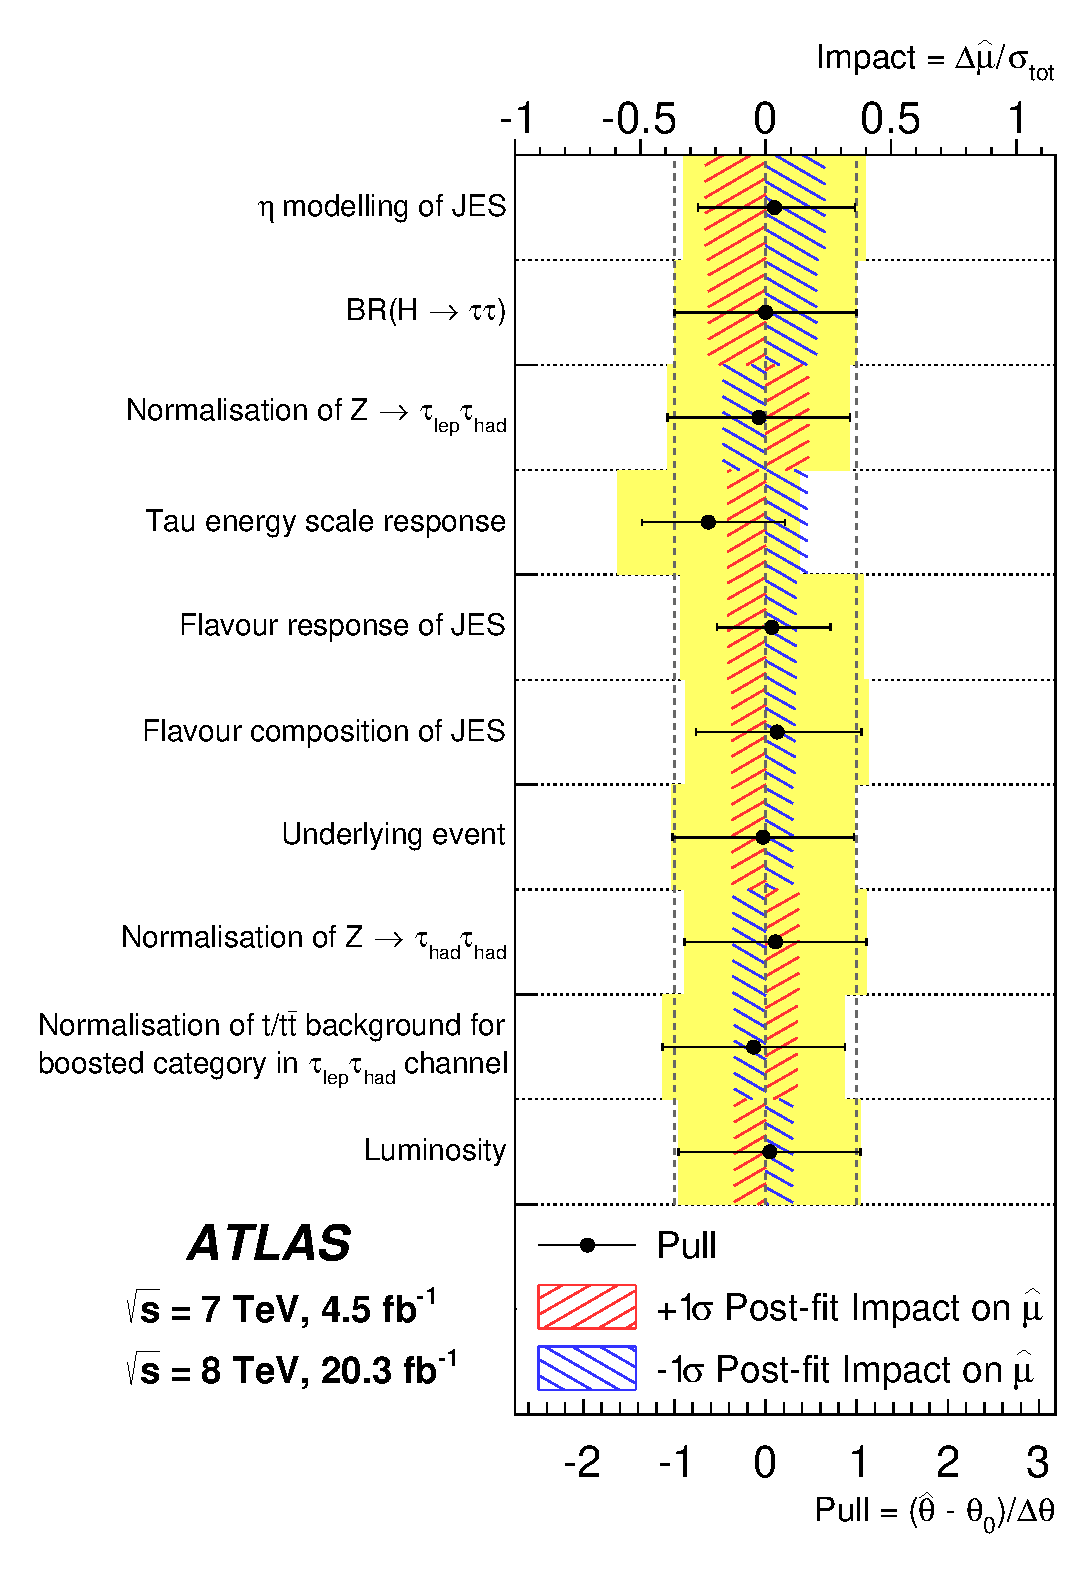
\includegraphics[width=0.90\textwidth]{figures/HIGG-2013-32/fig_07}
%%   \caption{Comparison of the impact and pull of the dominant individual systematic uncertainties on the absolute uncertainty on $\upmu$~\cite{HIGG-2013-32}.}
%%   \label{fig:results-uncertainties-2}
%% \end{figure}

\section{High score events in data}

Event displays of some of the most signal-like events in data in the VBF $\Htautaulh$ and $\Htautauhh$ analyses are shown in \cref{fig:results-eventdisplay-lh,fig:results-eventdisplay-hh}.

\begin{figure}[tp]
  \centering
  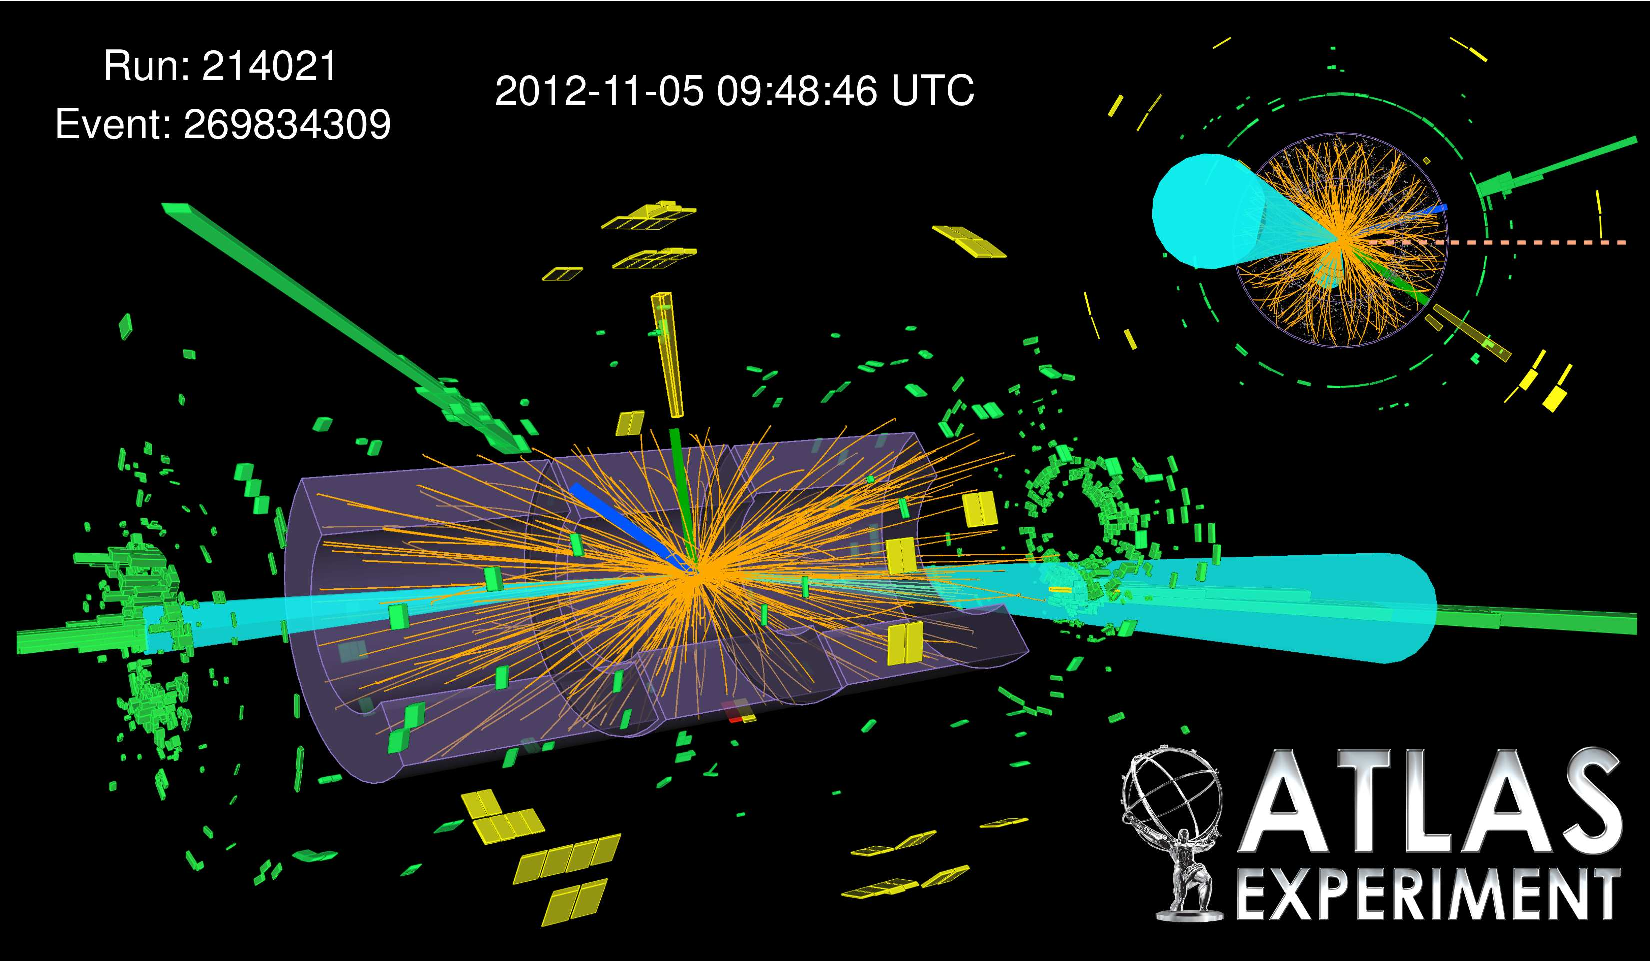
\includegraphics[width=0.80\textwidth]{figures/HIGG-2013-32/figaux_19}
  \caption{Display of one of the most signal-like events in the $\Htautaulh$ VBF category in data~\cite{HIGG-2013-32}. The blue track matched to the green cluster indicates an electron, the green track matched to the yellow cluster indicates a $\tauh$, the pink dotted line indicates the $\MET$ in the transverse plane, and the turquoise cones indicates the VBF jets. The reconstructed $\mMMC = 127$ GeV and $\mjj = 1.53$ TeV.}
  \label{fig:results-eventdisplay-lh}
\end{figure}

\begin{figure}[tp]
  \centering
  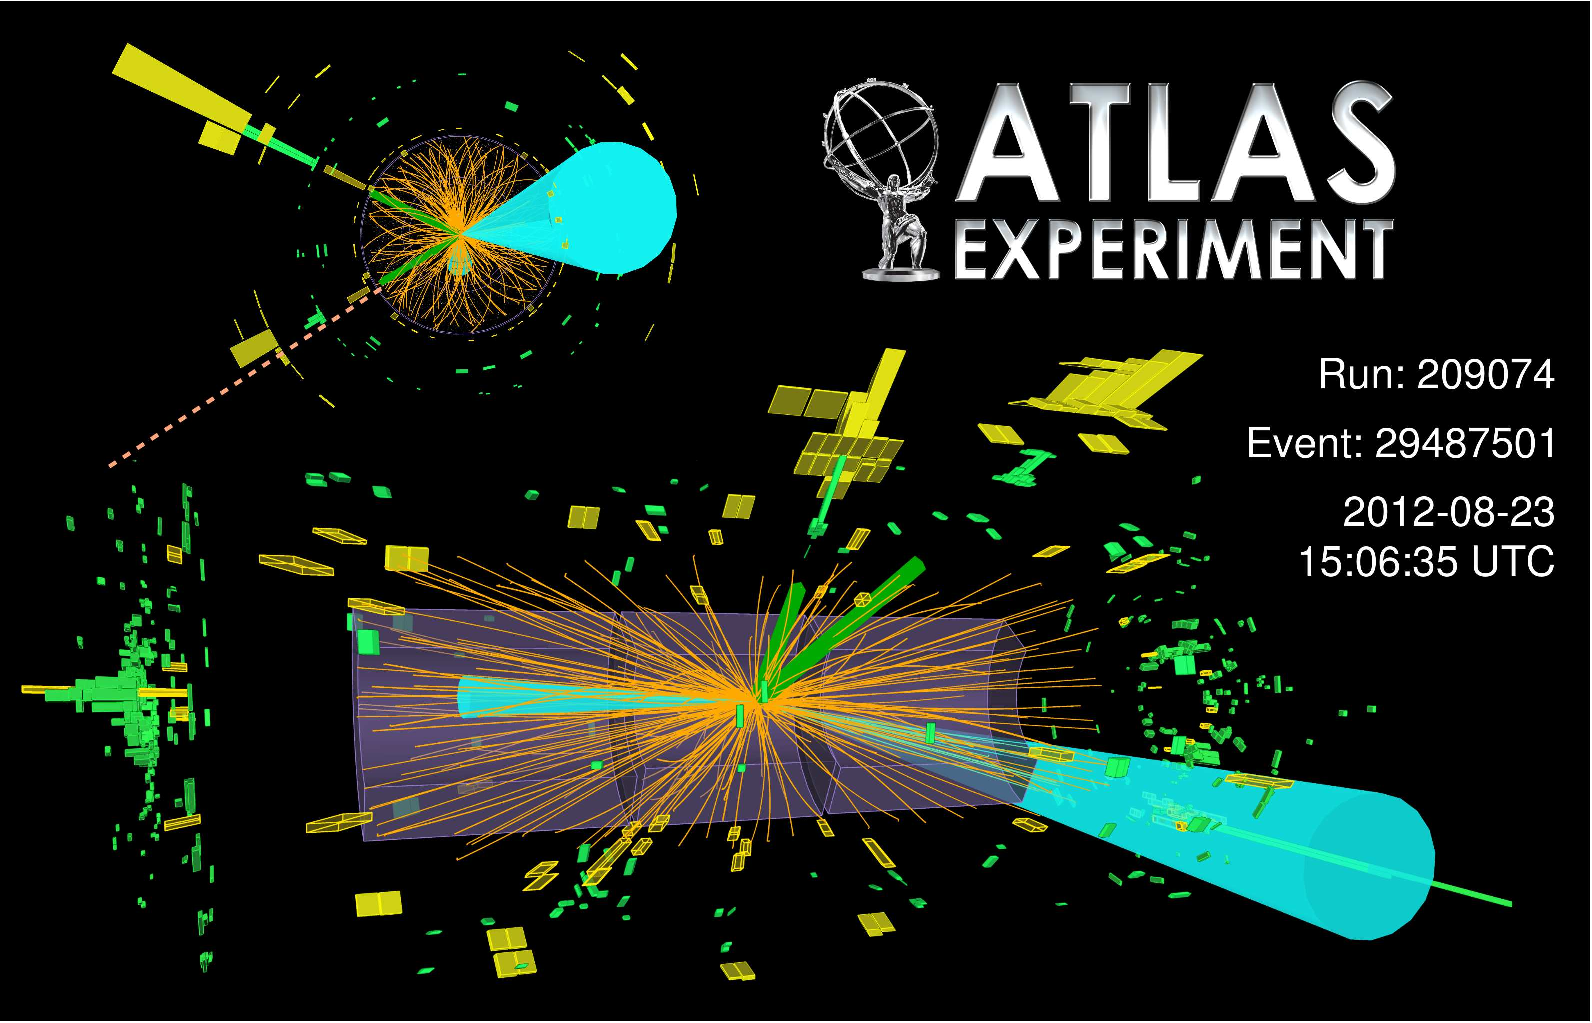
\includegraphics[width=0.80\textwidth]{figures/HIGG-2013-32/figaux_20}
  \caption{Display of one of the most signal-like events in the $\Htautauhh$ VBF category in data~\cite{HIGG-2013-32}. The green tracks matched to the yellow clusters indicate the $\tauh$, the pink dotted line indicates the $\MET$ in the transverse plane, and the turquoise cones indicates the VBF jets. The reconstructed $\mMMC = 123$ GeV and $\mjj = 1.02$ TeV.}
  \label{fig:results-eventdisplay-hh}
\end{figure}

